\documentclass{article}
\usepackage{graphicx}
\usepackage[utf8]{inputenc}
\usepackage{xeCJK}
\usepackage{amsmath}
\usepackage{bm}
\usepackage{minted}
\usepackage{hyperref}
\usepackage[dvipsnames]{xcolor}
\usepackage{parskip}
\usepackage{soul}
\usepackage{cancel}
\usepackage{ragged2e}
\usepackage[normalem]{ulem}

\hypersetup{hidelinks}

\title{Knuth–Morris–Pratt(KMP) 算法 \footnote{更多内容请访问:\url{https://github.com/SamZhangQingChuan/Editorials}}}
\author{张晴川\\\href{mailto:qzha536@aucklanduni.ac.nz}{\texttt{qzha536@aucklanduni.ac.nz}}}

\begin{document}
\maketitle

\section{题意}
设文本串为 $T(1\le |T| \le 10^5)$,模式串为 $S(1\le |S| \le 10^5)$,求 $S$ 在 $T$ 中的所有出现位置。下标均从 $1$ 开始。

例:$S = \texttt{14},T = \texttt{114514}$,那么匹配的末尾位置为 $\{3,6\}$


\section{算法}
首先我们考虑用一个没有出现过的字符 $\texttt{\#}$ 把 $\texttt{S}$ 和 $\texttt{T}$ 拼成一个串 $\texttt{S\#T}$,例如 $\texttt{14\#114514}$。

现在考虑对于位置 $\texttt{i}$,有哪些以它结尾的串等于相同长度的\textbf{前缀},以 $\texttt{i}$结尾的前缀本身除外。例如对于串 $\texttt{aba\#ababa}$,最后一个位置 $\texttt{i} = 9$ 的话,匹配的长度为$\{3,1,0\}$,分别对应 $\{\texttt{aba},\texttt{a},\epsilon\}$ \footnote{$\epsilon$ 表示空串},定义这样的串为以 $\texttt{i}$ 结尾的\texttt{border}。 

\paragraph{问题转化} 我们用 $\texttt{match(i,len)} = \texttt{true}/\texttt{false}$ 表示以 $\texttt{i}$ 结尾,长度为 $\texttt{len}$ 的串是否是 \texttt{border},用$\texttt{borders[i]}$ 表示以 $\texttt{i}$ 结尾,所有\texttt{border} 的集合。原问题可以转化为:对于多少位置 $\texttt{i}$,$\texttt{match(i,|S|)} = \texttt{true}$。

\dotfill     

\paragraph{如何求$\texttt{borders[i]}$} 首先我们可以发现 $\texttt{match(i,len)} = \texttt{true}$ 成立有两个条件:
\begin{enumerate}
\item $\texttt{match(i-1,len-1)} = \texttt{true}$
\item $\texttt{S[len]} = \texttt{S[i]}$
\end{enumerate}
\begin{center}
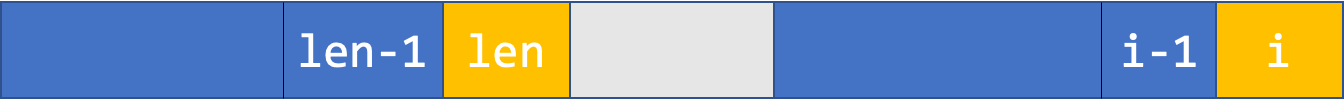
\includegraphics[width=8cm]{1.png}
\end{center}

于是我们可以枚举 $\texttt{borders[i-1]}$ 里的元素,如果下一位恰好和 $\texttt{S[i]}$ 匹配,那么就 $\texttt{+1}$ 就可以得到 $\texttt{borders[i]}$ 里的一个元素。最后加入 $0$ 即可。设 $n = |S|+|T|$,由于一共有 $n$ 个位置,每次最多枚举 $n$ 个元素,复杂度为 $O(n^2)$ ,需要加速。

\dotfill

\paragraph{更高效的表示方法}我们用 $\texttt{next[i]}$ 表示 $\texttt{borders[i]}$ 里最长的 \texttt{border}。假设 \texttt{len} 也是 \texttt{i} 的一个 \texttt{border},不难发现 \texttt{len} 也是 $\texttt{next[i]}$ 的 \texttt{border}。(参考下图,想想为什么)

\begin{center}
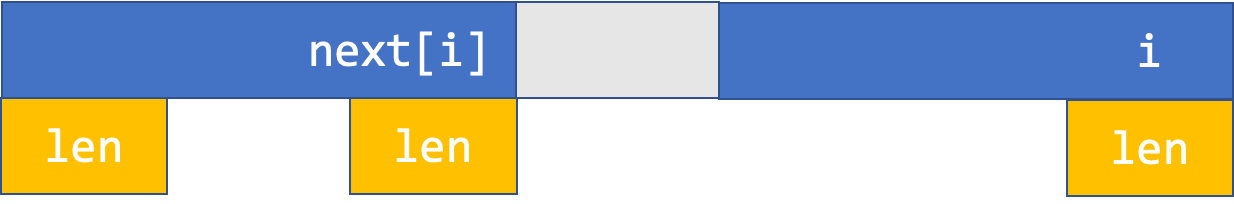
\includegraphics[width=8cm]{2.png}
\end{center}

所以除了 $\texttt{next[i]}$ 外,其余元素都是 $next[i]$ 的 $border$,于是可以得到:
    $$\texttt{borders[i]} = \{\texttt{next[i]}\} \cup \texttt{borders[next[i]]}$$
展开写的话就是:
    $$\texttt{borders[i]} = \{\texttt{next[i]},\texttt{next[next[i]]},\ldots,0\}$$
另外根据定义, $\texttt{borders[1]} = \{0\}$。

\dotfill

\paragraph{递推求解} 由上述解释,只需要求出 \texttt{next[i]},就可以得到整个 \texttt{borders[i]}。如果知道了\texttt{borders[i]},$\texttt{next[i+1]}$就等于\texttt{borders[i]}里从大到小第一个可以转移到 $\texttt{i+1}$ 的元素再加 $1$  。如果全部无法转移,那么 $\texttt{next[i+1]} = 0$。

\dotfill

\paragraph{完全解决} 

在求出所有 $\texttt{next[i]}$ 之后,只需要计算有哪些位置的 $\texttt{next[i]} = |S|$ 即可。

\section{习题}
\begin{enumerate}
\item 实现 KMP 算法
\item \href{https://loj.ac/problem/2246}{「NOI2014」动物园}
\item 以同样思路分析 AC 自动机的算法。

\end{enumerate}

\newpage
\section{核心代码}
\inputminted[linenos,autogobble]{cpp}{kmp.cpp}



\end{document}
